\documentclass{bmvc2k}

%% Enter your paper number here for the review copy
% \bmvcreviewcopy{??}

% \usepackage[brazilian]{babel}
\usepackage[utf8]{inputenc}

\title{Seleção de pixels com cores \\similares em imagem e vídeo}

% Enter the paper's authors in order
% \addauthor{Name}{email/homepage}{INSTITUTION_CODE}
\addauthor{Pedro Garcia}{drogpe@gmail.com}{1}
%\addauthor{}{}{1}

% Enter the institutions
% \addinstitution{Name\\Address}
\addinstitution{
  Departamento de Ci\^encia da Comptuta\c{c}\~ao\\
  Universidade de Bras\'{\i}lia\\
  Campus Darcy Ribeiro, Asa Norte\\
  Bras\'{\i}lia-DF, CEP 70910-900, Brazil,  
}

\runninghead{Garcia}{Computer Vision Assignment -- \today}

% Any macro definitions you would like to include
% These are not defined in the style file, because they don't begin
% with \bmva, so they might conflict with the user's own macros.
% The \bmvaOneDot macro adds a full stop unless there is one in the
% text already.
\def\eg{\emph{e.g}\bmvaOneDot}
\def\Eg{\emph{E.g}\bmvaOneDot}
\def\etal{\emph{et al}\bmvaOneDot}

%-------------------------------------------------------------------------
% Document starts here
\begin{document}

\maketitle

\begin{abstract}
   Este é o relatório do Projeto Demonstrativo 1 da disciplina de Princípios de Visão Computacional. O objetivo do projeto é criar um programa que retorna os dados de um pixel selecionado em uma imagem. O programa também destaca pixels com cor similar, tanto em imagens quanto em vídeos/webcam. Após o desenvolvimento do programa, ele foi testado e funcionou perfeitamente.
\end{abstract}

%-------------------------------------------------------------------------
\section{Introdução}
\label{sec:intro}

Este projeto demonstrativo tem como objetivo implementar um programa que faça uso de funções básicas do openCV, como abrir imagens e vídeos e extrair informação de cores dos seus pixels. Ele foi dividido em 4 requisitos:
\begin{enumerate}
    \item Ao abrir uma imagem, o usuário clica sobre um ponto nela e é exibido no terminal a coordenada do pixel e os seus valores de cor RGB, ou o seu brilho caso a imagem esteja em escala de cinza;
    \item Quando o usuário clica sobre uma imagem, destacar todos os pixels com cor semelhante ao pixel clicado, colorindo-os de vermelho;
    \item Procedimento análogo ao item 2, mas em vez de abrir uma imagem o programa deve abrir um vídeo;
    \item Procedimento análogo aos itens 2 e 3, mas dessa vez a fonta das imagens deve ser a webcam.
\end{enumerate}

Para o desenvolvimento desse programa foi necessário aprender as funções básicas do OpenCV~\cite{opencv}. A linguagem de programação escolhida para a implementação foi Python, devido à simplicidade do problema e grande popularidade da linguagem em programas similares.

\section{Metodologia}
\label{sec:met}

O primeiro passo foi criar uma função de callback para eventos do mouse, uma vez que a principal forma de interação do usuário com o programa é através do mouse. A função \textit{mouseClickCallback()} detecta o evento do click do botão esquerdo e exibe no terminal as coordenadas do pixel e os valores RGB da sua cor, ou o seu brilho, caso a imagem esteja em escala de cinza.

Para determinar se a imagem está em escala de cinza, foi criada a função \textit{isGray()}. Ela gera 3 matrizes a partir da imagem, cada uma contendo os valores de cor de uma das componentes RGB. Depois são criadas mais 3 matrizes que são as diferenças 2 a 2 entre matrizes R, G e B. Em seguida toma-se o maior valor dentre essas matrizes e ele é comparado com uma tolerância. Caso ele seja maior que a tolerância, a imagem é considerada colorida e a função retorna \textit{False}. Caso contrário, a imagem é considerada em escala de cinza e a função retorna \textit{True}.

A função que destaca os pixels de cor semelhante é \textit{hlSimilarPixels()}. Ela começa por gerar as 3 matrizes com as componentes de cor da imagem (decidiu-se fazer isso mesmo para a imagem em escala de cinza). Em seguida é gerada uma matriz com a distância euclidiana entre os valores das 3 matrizes e o valor RGB do pixel clicado. Depois é gerada uma máscara que separa as entradas da matriz onde a distância é maior ou menor que 13, conforme a especificação do projeto. Por fim, aplica-se a máscara numa imagem que é cópia da original e define-se os pixels não mascarados como vermelhos.

Quando o programa está no modo imagem, chama-se a função \textit{picture()}, que abre e exibe a imagem, chama a função \textit{isGray()} e espera pela entrada do usuário.

O modo de vídeo/webcam é executado pela função \textit{video()}, mudando apenas o parâmetro relativo à entrada. Essa função abre o vídeo e vai exibindo os frames 1 a 1. Caso o usuário já tenha clicado em um pixel, ela começa a chamar \textit{hlSimilarPixels()} para cada frame antes de exibí-lo.

\section{Resultados}
\label{sec:res}

Pode-se ver a saída do programa para imagens de entrada nas figuras \ref{fig:cor} e \ref{fig:gray}.

\begin{figure}[htpb]
\begin{center}
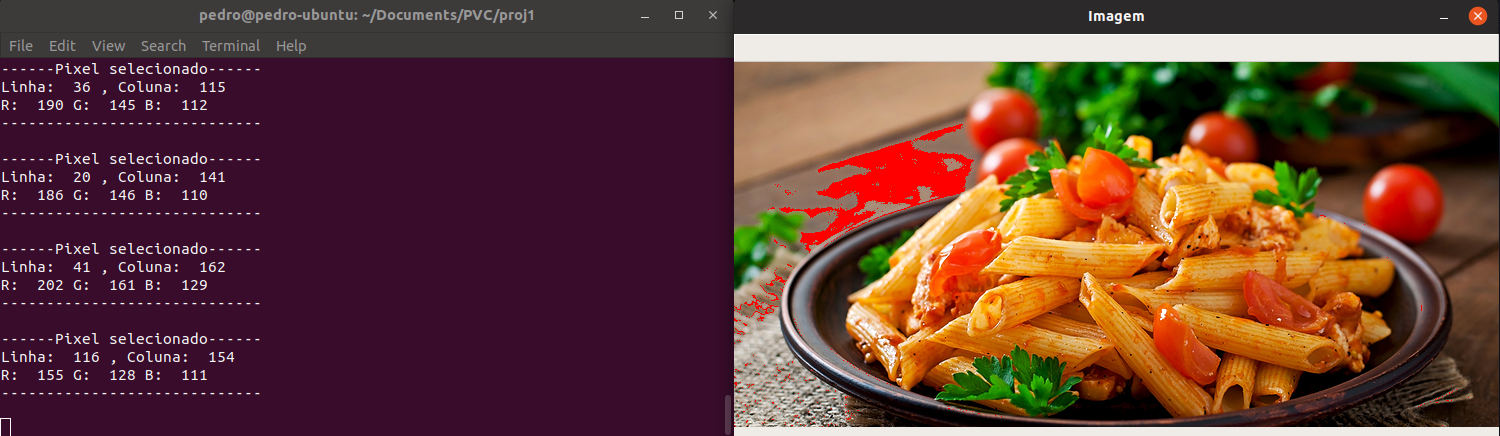
\includegraphics[width=0.8\textwidth]{Figs/img2.png}
\end{center}
   \caption{Seleção de pixels em imagem colorida.}
   \label{fig:cor}
\end{figure}

\begin{figure}[htpb]
\begin{center}
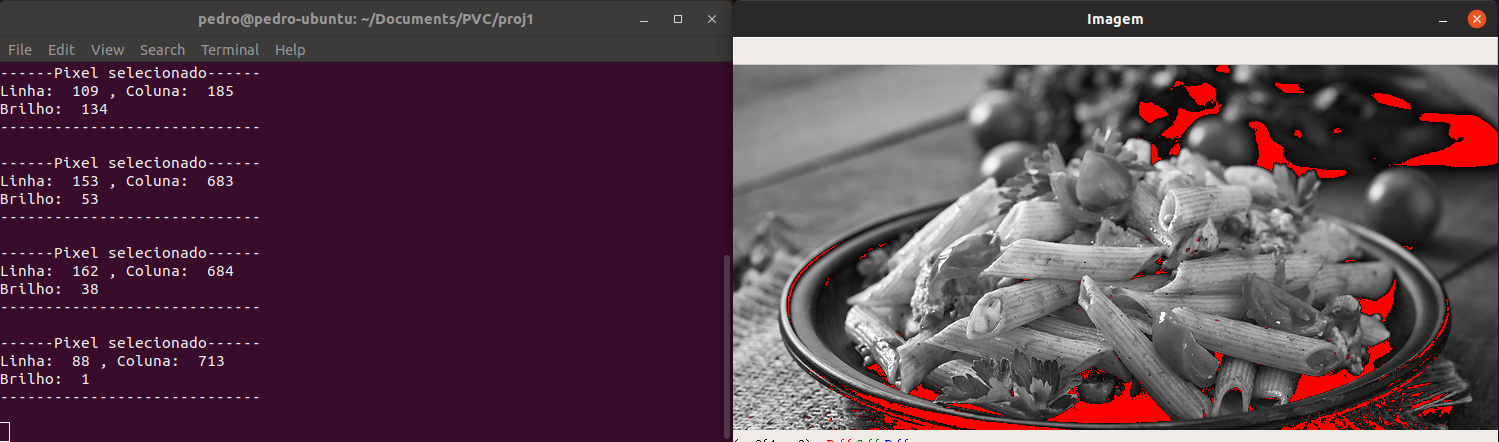
\includegraphics[width=0.8\textwidth]{Figs/img1.png}
\end{center}
   \caption{Seleção de pixels em imagem em escala de cinza.}
   \label{fig:gray}
\end{figure}

As outras funções do programa também funcionaram adequadamente. Decidiu-se não colocar imagens aqui porque não faz muito sentido colocar uma \textit{screenshot} de um vídeo. 

\section{Discussão e conclusões}
\label{sec:concl}

Vê-se o destaque de pixels de cor similar funcionando para imagens coloridas e em escala de cinza. Observa-se também a saída no terminal com as informações do ponto clicado, mostrando as componentes RGB na Figura \ref{fig:cor} e o brilho na Figura \ref{fig:gray}.

Pode-se dizer que 13 é uma tolerância pequena, uma vez que cores que um ser humano consideraria idênticas não são selecionadas.


\bibliography{refs}
\end{document}
